\documentclass[11pt,letterpaper]{article}
\usepackage[margin=0.7in]{geometry}
\usepackage[T1]{fontenc}
\usepackage{lmodern,microtype,graphicx,booktabs,amsmath,xcolor,fancyhdr}
\usepackage[hidelinks]{hyperref}
\usepackage[font=small,labelfont=bf]{caption}
\setlength{\parindent}{0pt}\setlength{\parskip}{7pt}\setlength{\emergencystretch}{4em}
\pagestyle{fancy}\fancyhf{}\fancyhead[L]{Cross-language attention}
\fancyhead[R]{Independent research manuscript}\fancyfoot[L]{28 October 2026 --- not peer reviewed}
\fancyfoot[R]{\thepage}\setlength{\headheight}{14pt}
\begin{document}
{\LARGE\bfseries English history does not improve\\every topic holdout\par}
\vspace{8pt}
{\large Lagged forecast transfer across fixed Wikipedia titles\par}
{\small James N. Jean IV \quad Independent, AI-assisted research example \quad 28 October 2026\par}
\section*{Executive summary}
An editor considering another language's traffic as a forecasting input needs evidence that the added signal transfers to the topics and language of interest. In this retrospective daily benchmark, fast English lags lowered 2025 RMSLE from 0.2964 to 0.2933 across three held Spanish topics. Across four held Japanese topics, they raised it from 0.3017 to 0.3052. Three of those four Japanese pages improved individually; a larger loss on the Tsunami page reversed the equal-page mean.

The fast-English held-topic paired MSLE differences were $-0.001826$ in Spanish and $+0.002107$ in Japanese. Their conditional 95\% common-month intervals both crossed zero: $[-0.003551,\allowbreak +0.000118]$ and $[-0.001876,\allowbreak +0.007394]$. These point estimates do not establish a general gain or loss. A majority of page-level wins is also insufficient to establish useful average transfer.

\begin{center}\small
\begin{tabular}{lrrrr}\toprule
Parameter-selection role & Pages & Own history & Fast English & Slower English\\\midrule
Spanish development & 9 & 0.2327 & 0.2264 & 0.2300\\
Spanish held topics & 3 & 0.2964 & 0.2933 & 0.2978\\
Japanese development & 10 & 0.2202 & 0.2167 & 0.2206\\
Japanese held topics & 4 & 0.3017 & 0.3052 & 0.3068\\\bottomrule
\end{tabular}
\captionof{table}{2025 page-balanced RMSLE; lower is better. Every page has 365 test dates. RMSLE is the square root of equal-page mean squared log error, not a percentage. Development/held labels concern earlier hyperparameter selection; all rows use the held test year.}
\end{center}

Retain an own-history comparator and examine the target language and held topics separately. Before live use, obtain historical API publication vintages and evaluate a new protected period. The current data are historical snapshots retrieved later, with a two-day input-availability assumption. They do not validate prospective forecasting.

This study retains 69,300 daily source counts, 567 validation fits, 78 final refits, 47,450 test predictions and all eight paired comparisons. Independent checks reconstruct source joins, coefficients, predictions, metrics, resampling and plotted values. The contribution is a transparent bounded comparison and its failure case; it does not claim a new forecasting algorithm, causal attention flow or realized operational savings.

\newpage
\section*{1. Data, scope and information timing}
The Wikimedia Analytics API supplies aggregate daily all-access counts classified as user traffic for fixed English, Spanish and Japanese titles, from 1 January 2022 through 31 December 2025. Counts measure content requests, not distinct people, geography or language fluency. Bot classification is imperfect; redirects and title histories can affect interpretation. Analytics data and Wikidata structured metadata are supplied under CC0 [1--3]. No article prose, editor identities or individual browsing records were requested.

The initial twelve convenience topics were Earth, Moon, Mars, Sun, Volcano, Earthquake, Tsunami, Artificial intelligence, Machine learning, Climate change, Olympic Games and Solar eclipse. An original source/coverage gate failed. Before fitting or inspecting forecast-outcome summaries, a retained amendment added Water, Photosynthesis, Computer and Music as development topics, and corrected the move-log exclusion interval to 2022--2025. The original snapshot, failed gate and amendment remain inspectable. This was a source-driven design change, not a pretense that the original panel passed unchanged.

The revised snapshot contains 289 response records, 48 current title identities and 32 candidate target-language pairs. Twenty-six pairs pass unchanged coverage minimums; six remain excluded. Excluded pairs are Spanish Climate change, Japanese Climate change, Spanish Earth, Spanish Earthquake, Japanese Earthquake and Spanish Moon. Spanish Climate change fails current-title resolution/coverage; the other five pairs have an in-period title-move event. Title-filtered move logs provide bounded lineage checks, not exhaustive historical alias equivalence. No aliases are combined into concept-wide totals.

Only the nine eligible Spanish development topics supply hyperparameter-selection outcomes. Moon, Tsunami, Machine learning and Olympic Games remain topic holdouts; three pass Spanish eligibility and four Japanese eligibility. Japanese supplies no selection outcomes. Every final page model is fitted to its own pre-2025 history. These are holdouts for \emph{parameter selection}, not cold-start predictions for unseen pages.

Predictions for UTC date $t$ use observed counts dated at most $t-2$, plus known calendar fields. Labels for each fitting origin stop two days before that origin. During validation or test, earlier outcomes from that same period may become lag features once their delay has elapsed; fitted coefficients stay fixed. Exact historical API availability/revisions are unavailable, so the two-day delay is an assumption rather than an observed publication guarantee.

\section*{2. Models and evaluation target}
All three ridge families use own-page $\log(1+v)$ at lags 2, 7, 14 and 28 and the mean log count over lags 2--8, six weekday indicators and annual sine/cosine terms with a 365.25-day cycle. Fast English adds its corresponding five lag features. Slower English instead adds lags 7, 14, 21 and 35 and the mean over lags 7--13. Calendar/history structure motivates this compact design; no empirical feature-importance or causal rationale is claimed.

All methods share eligible dates requiring every relevant count and the maximum 35-day history. Missing values are never replaced by zero. The two simple comparators are $v_{t-7}$ and $(v_{t-7}+v_{t-14}+v_{t-21}+v_{t-28})/4$. Their predictions use counts in original units.

\newpage
\section*{3. Finite selection and numerical fitting}
Each ridge fit standardizes predictors using fitting rows only, then minimizes
\[
\frac{1}{n}\sum_i\bigl(\log(1+v_i)-a-z_i^\mathsf{T}b\bigr)^2+\lambda\lVert b\rVert_2^2,
\]
with an unpenalized intercept. Penalties are selected by equal page/fold mean MSLE across three forward 2024 folds: January--April, May--August and September--December. Training expands from 2022 to the two-day cutoff before each fold. Exact ties choose the smaller penalty.

The original five penalties, 0.01 through 100 in powers of ten, produced 405 fits; all three winners reached the lower boundary. A documented validation-only extension added 0.001 and 0.0001 before first test inference, retaining every original trial unchanged. The final 21 settings produced 567 successful fits and 69,174 validation predictions. Selected penalties were 0.001 (own), 0.01 (fast) and 0.001 (slower), interior to that finite pool. They are not global generalization optima.

\begin{center}
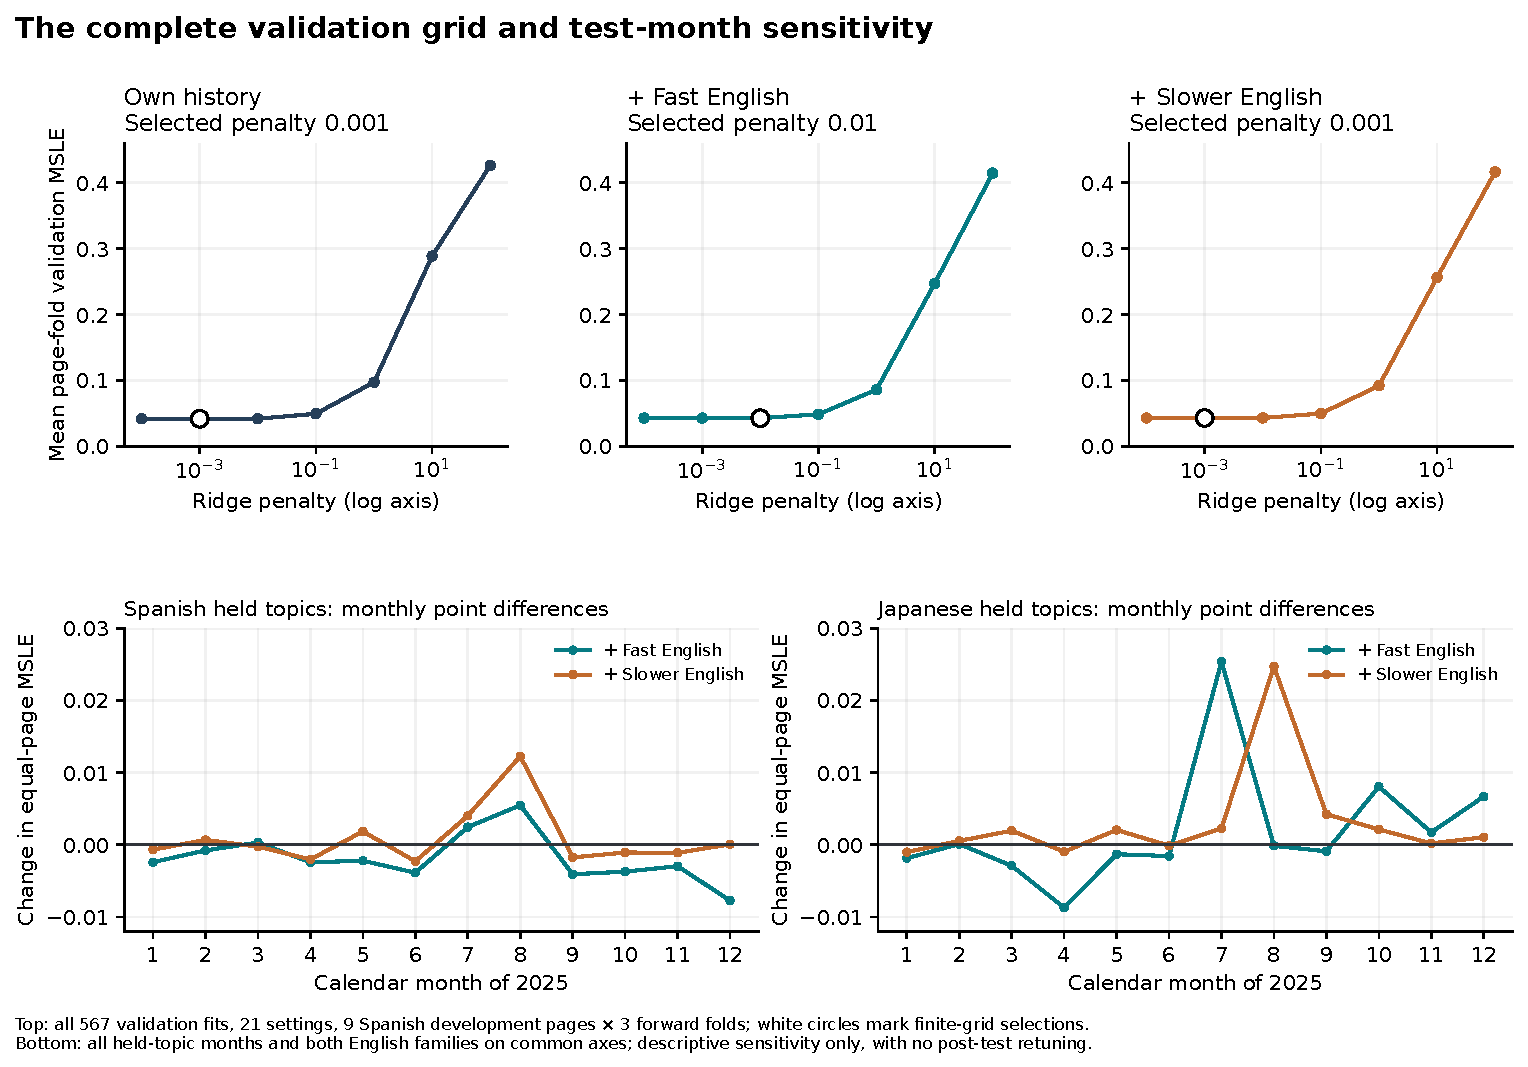
\includegraphics[width=\linewidth]{images/03_search_and_months.pdf}
\captionof{figure}{Complete selection evidence and held-topic month sensitivity. Upper panels use only Spanish development validation; lower panels describe every held test month on common axes. Monthly reversals do not support a stable universal advantage or identify their causes.}
\end{center}

All 645 ridge fits passed independent scalar objective/gradient, positive-definite Hessian and augmented-QR checks: maximum gradient $2.58\times10^{-14}$, minimum Hessian eigenvalue 0.00492 and maximum QR coefficient difference $9.66\times10^{-14}$. This supports the fitting objective, not generalization. Final models, transforms, rules, source hashes and code were committed before first test inference (freeze \texttt{5a446198de1f}).

\newpage
\section*{4. Predictive results}
For page $p$, MSLE averages $(\log(1+\widehat v)-\log(1+v))^2$ across dates. Group MSLE averages page MSLEs equally; reported group RMSLE is its square root, rather than the mean of page RMSLEs. Negative raw predicted logs are retained, then clipped to zero before exponentiation; overflow is rejected, with no upper prediction cap. All three families and both baselines are retained.

\begin{center}
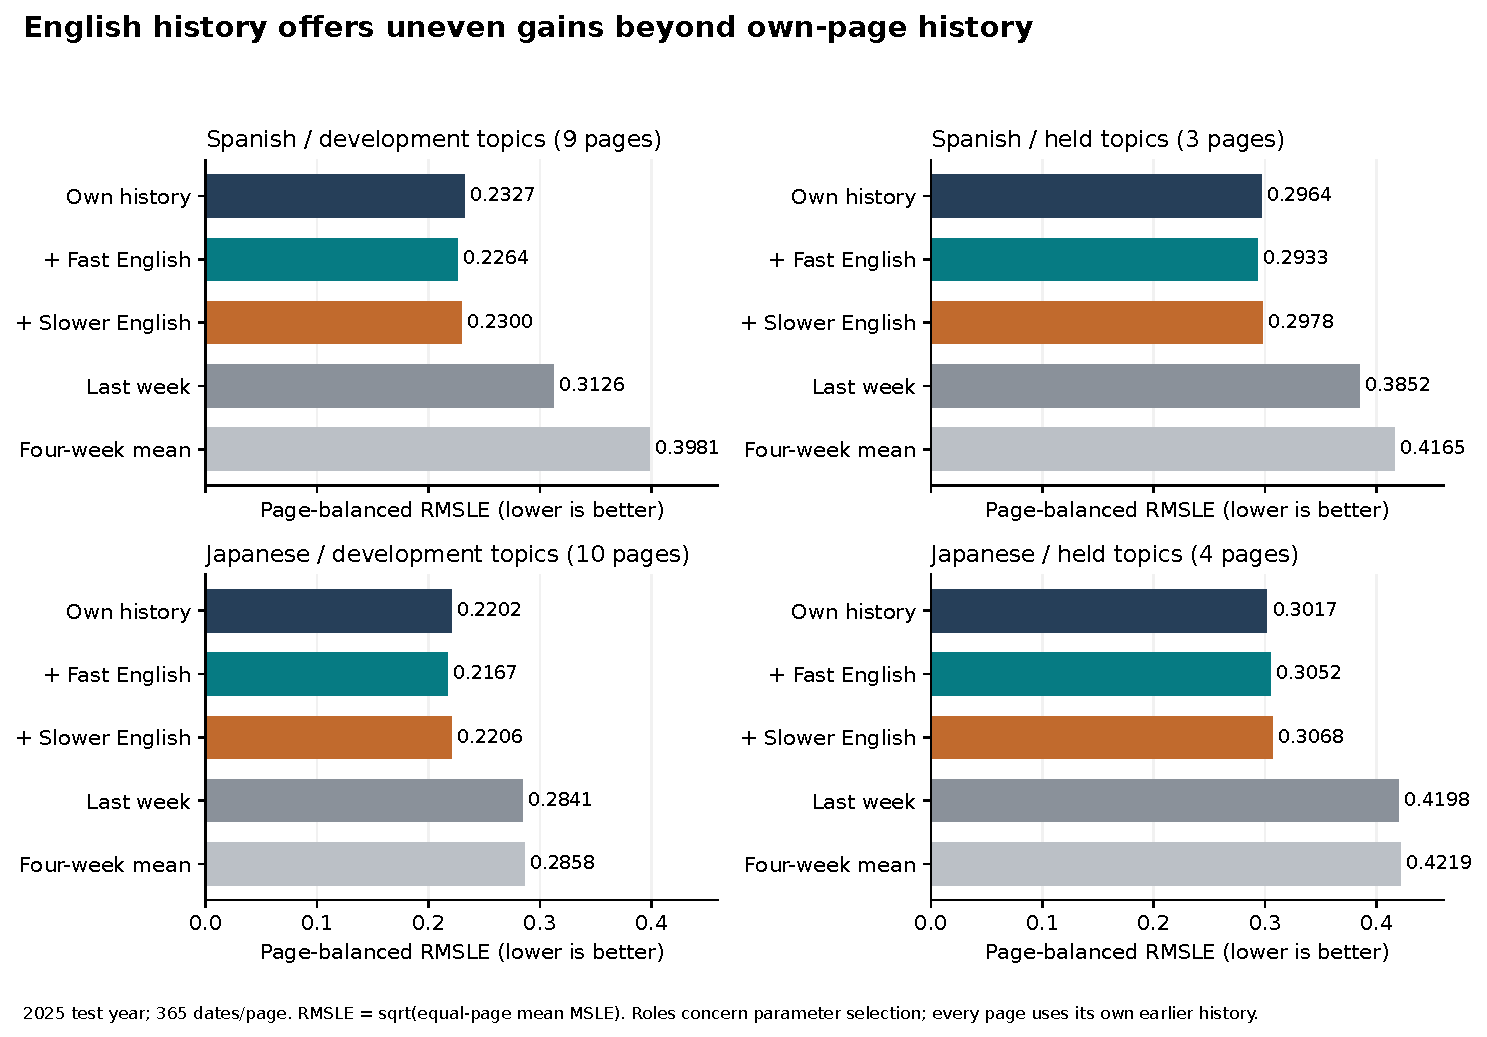
\includegraphics[width=\linewidth]{images/01_predictive_comparison.pdf}
\captionof{figure}{Full 2025 method comparison. Every group uses 365 dates per page and the same eligible dates across methods. Bars begin at zero. Smaller differences between ridge families remain visible through numeric labels and the paired comparison in Figure 3.}
\end{center}

Across all twelve Spanish pages, own/fast/slower RMSLE was 0.2501/0.2448/0.2487; across fourteen Japanese pages it was 0.2462/0.2453/0.2483. Those aggregate rows conceal the Japanese held-topic loss. Fast English improved 10 of 12 Spanish pages and 10 of 14 Japanese pages; neither count substitutes for magnitude-sensitive, role-specific error.

Raw-unit losses answer different questions. On Japanese held topics, fast English reduced mean page MAE from 65.66 to 64.28 views/day while increasing RMSLE; mean page MSE rose from 245,565.2 to 246,524.5 views$^2$. The exported tables also retain raw RMSE and seasonal MASE, using each page's fitting-period lag-seven absolute-error scale. No cost function, staff allocation, monetary saving or reader benefit was measured.

\newpage
\section*{5. Paired differences and conditional uncertainty}
The paired bootstrap draws 12 calendar months with replacement 2,000 times per language/role group, sharing the sampled months across pages and both English comparisons. Seed 20261028 and the PCG64 generator are fixed; all 16,000 comparison draws and month indices are retained. Each draw divides by its sampled date count within page, then averages pages equally. Intervals are 2.5th/97.5th percentiles, conditional on this fixed convenience panel and its twelve months. They do not estimate independent-topic, worldwide-reader or causal uncertainty, and no multiplicity-adjusted discovery claim is made.

\begin{center}
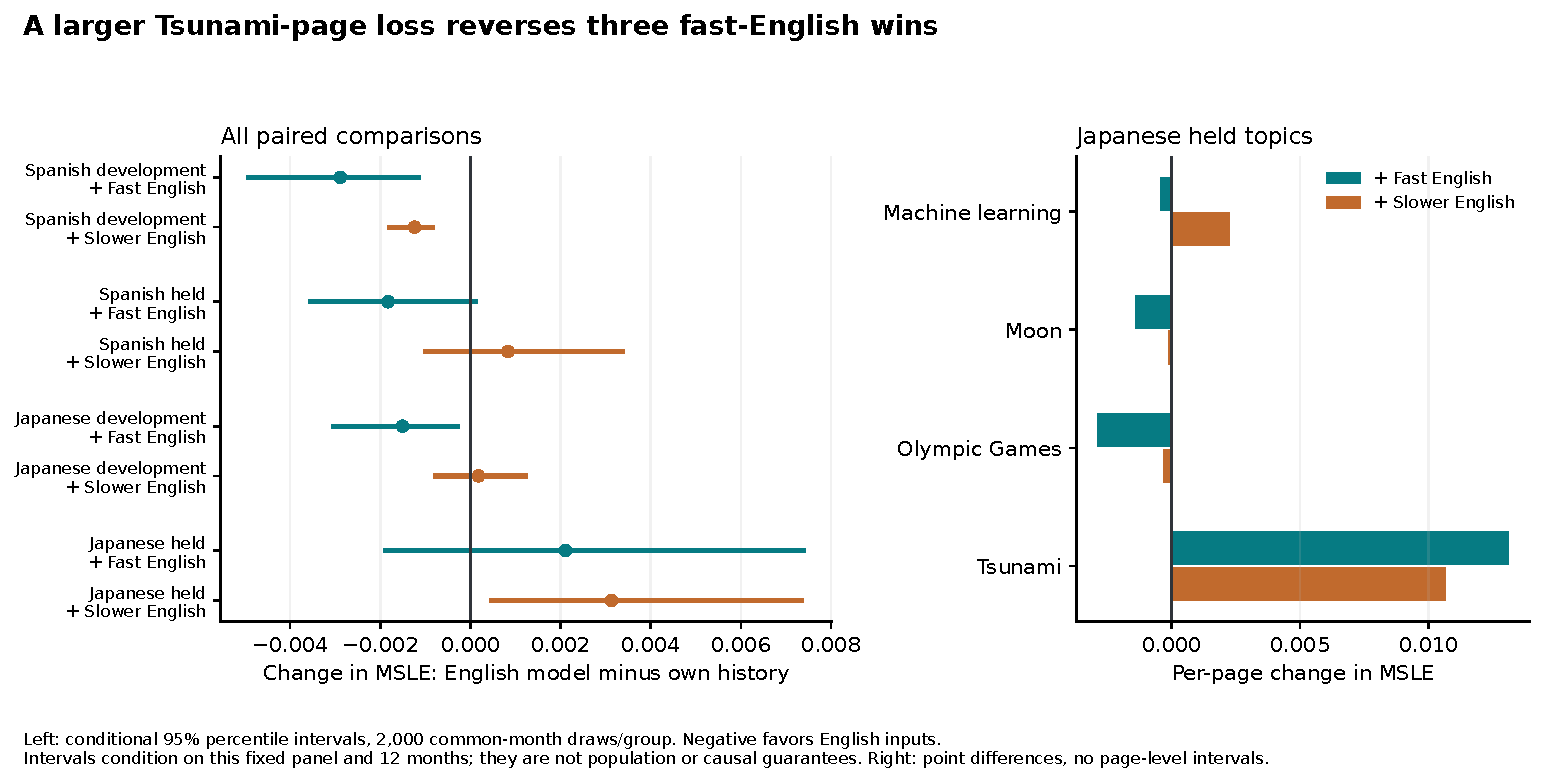
\includegraphics[width=\linewidth]{images/02_paired_transfer.pdf}
\captionof{figure}{All eight English-minus-own MSLE differences and conditional intervals. Negative favors English features. On Japanese held topics, three small fast-English improvements are outweighed by the Tsunami loss; right-hand bars are page-level point differences without per-page intervals.}
\end{center}

Fast English's Japanese held-topic differences were $-0.000423$ (Machine learning), $-0.001386$ (Moon), $-0.002886$ (Olympic Games) and $+0.013124$ (Tsunami). Their average was $+0.002107$. This arithmetic explains the aggregate reversal without attributing a cause to events, reader behavior or information transmission.

Slower English's held-topic mean difference was $+0.000834$ in Spanish, with interval $[-0.000989,\allowbreak +0.003365]$, and $+0.003128$ in Japanese, with interval $[+0.000470,\allowbreak +0.007340]$. The latter interval stays positive under this conditional resampling rule. All development-topic intervals and both held-topic families remain in the figure and exported table; test results did not select a method for suppression or retuning.

\newpage
\section*{6. Reproducibility, limits and next evidence}
The public repository retains eligible source snapshots and request/hash manifests; original source-gate failure and pre-fit amendment; all candidate models, transforms, predictions, fit attempts and metrics; the validation extension; the committed final freeze; all test rows and bootstrap draws; and the original analytical figures. Independent SQL/source reconciliation checks every count, title identity, reuse byte and pair-date eligibility. Independent coefficient and scalar-prediction checks import no primary fitting or metric helper. Absolute/relative comparison tolerances remain $10^{-7}$/$10^{-9}$.

The offline replay rebuilds ingestion, all 567 validation fits, all 78 final refits, every prediction and metric, the bootstrap and figures in a temporary directory. It compares scientific values with retained outputs. Per-run provenance hashes are checked internally; cross-platform newline serialization, run timings and the temporary replay commit marker are not treated as scientific discrepancies. The original 405-model archive and historical pre-test freeze remain separately verified. Pinned Python dependencies and eight scientific contract tests accompany the replay. The repository's current CI and release evidence, rather than this document alone, establish which revision passed on Linux.

These finite checks cannot establish exhaustive correctness, scientific novelty or prospective validity. The panel is small and conveniently chosen, languages/topics share shocks, source exclusions alter coverage, and only one test year is available. Current sitelinks and bounded title logs do not certify complete historical concept equivalence. Request counts can include classification error; historical API publication vintages are absent. Fitting each page's own history tests transfer of a selection rule, not zero-data transfer. Log-scale accuracy may conflict with operationally relevant raw errors. Twelve resampled months provide limited conditional uncertainty and no independent population guarantee.

Cross-language predictors are established prior work: Xie, Johnson and Gomez discuss other language editions and geographies for predicting Wikipedia traffic [4]. This benchmark does not reproduce their event-impact estimators or claim to invent that idea. Its evidence supports a narrower recommendation: keep the own-history model, report target-language and held-topic losses alongside page-level wins, and avoid assuming that adding English history consistently improves a new editorial target. A new protected period with actual publication-vintage capture and an explicit operational loss is the next useful evaluation.

\section*{Sources and availability}
\small
[1] Wikimedia Foundation. \emph{Analytics API: access policy}. API data licensing and sequential identified requests. \href{https://doc.wikimedia.org/generated-data-platform/aqs/analytics-api/documentation/access-policy.html}{Official access policy}. Accessed 28 October 2026.

[2] Wikimedia Foundation. \emph{Analytics API: page views}. Request definition, redirect treatment and traffic classification. \href{https://doc.wikimedia.org/generated-data-platform/aqs/analytics-api/concepts/page-views.html}{Official concepts documentation}. Accessed 28 October 2026.

[3] Wikidata contributors. \emph{Wikidata: licensing}. Structured-data terms. \href{https://www.wikidata.org/wiki/Wikidata:Licensing}{Official licensing page}. Accessed 28 October 2026.

[4] Xiaoxi Chelsy Xie, Isaac Johnson and Anne Gomez. 2019. \emph{Detecting and Gauging Impact on Wikipedia Page Views}. \href{https://doi.org/10.48550/arXiv.1903.10670}{arXiv:1903.10670}. Related DOI: 10.1145/3308560.3316751.

Code, eligible data, detailed limitations and all checks: \url{https://github.com/S3R3Bii/cross-language-attention}. This is an independent, AI-assisted research manuscript, shared on GitHub with its evidence. It has not been peer reviewed or accepted for formal publication. Source papers, private records and unrelated formal-publication projects are excluded.
\end{document}
